\section{Experimental Methodology}
\label{sec:methodology}
\authoritativeDatasetTable
\subsection{Questions}
We ask: (Q1) When does the prefix topology with its covering frontier improve
over the matched LNG system? (Q2) Which effects come from block depth and
controlled topology changes? (Q3) Which profile counters explain these effects?
(Q4) How well does a query-calibration-free plan transfer relative to a frozen
manual candidate set? (Q5) What construction time and resources do
GPU-assisted overlays require?

\subsection{Execution Environment}
The experiment host uses two Intel Xeon Platinum 8360Y processors (72 physical
cores, 144 logical CPUs) and an NVIDIA L20 with 46,068 MiB reported device
memory. Queries use 100 CPU workers. The recorded host runs CentOS 7
with NVIDIA driver 550.54.14. The artifact manifests retain the hardware
snapshot, binary hashes, per-case backends, and GPU-idle checks. GPU acceleration is used for construction; query execution runs on the CPU.

\subsection{Datasets and Workloads}
We reuse the repository's preprocessed vector and integer-label datasets,
evaluating L2 distance on the stored floating-point coordinates. Canonical
tries sort stored label IDs in ascending order. The development dataset is Amazon with $602{,}453$ vectors of dimension 768 and
$482{,}387$ observed label groups.  Each Amazon workload contains 1,000 queries, uses
$K=10$, and has exact containment ground truth.  The measured mean
selectivities are 0.499249\%, 0.903055\%, 5.038117\%, 9.906615\%, 30.027242\%,
60.047491\%, 80.023699\%, 95.019781\%, and 99.000600\%.  Genome, Reviews, and
VariousImg are held out for the automatic-policy study; their exact workload
directories and fingerprints are recorded in the artifact manifest.
The 99\% Amazon workload contains 697 empty predicates and 303 singleton
predicates $\{1\}$.  The empty-predicate path is validated separately before timing.

The 0.5\%, 1\%, and 10\% batches reuse existing predicate files;
their mean query-label counts are 5.939, 5.763, and 3.396. The 5\%,
30\%, and 60\% batches raise the mean coverage of source batches by
replacing selected predicates with the frequent singleton $\{1\}$.
The 80\% and 95\% batches use the same construction and query vectors
from a 75\% source batch. Label 1 covers 96.702\% of the database, so
the 99\% batch mixes it with the empty predicate. These are batch-mean
selectivities: for example, individual queries in the 5\% batch range
from 0.0033\% to 96.702\%. Predicate composition and selectivity vary
together, so the sweep characterizes these workload families.
Figure~\ref{fig:query-composition} separates predicate size from individual
selectivity. An independent label-only pass recomputes the eligible counts
of all 9,000 queries and agrees with the saved coverage profiles; every
query has at least 20 eligible vectors. All base and query label rows in
these files are duplicate-free, so predicate size equals distinct-label count.

\begin{figure*}[t]
\centering
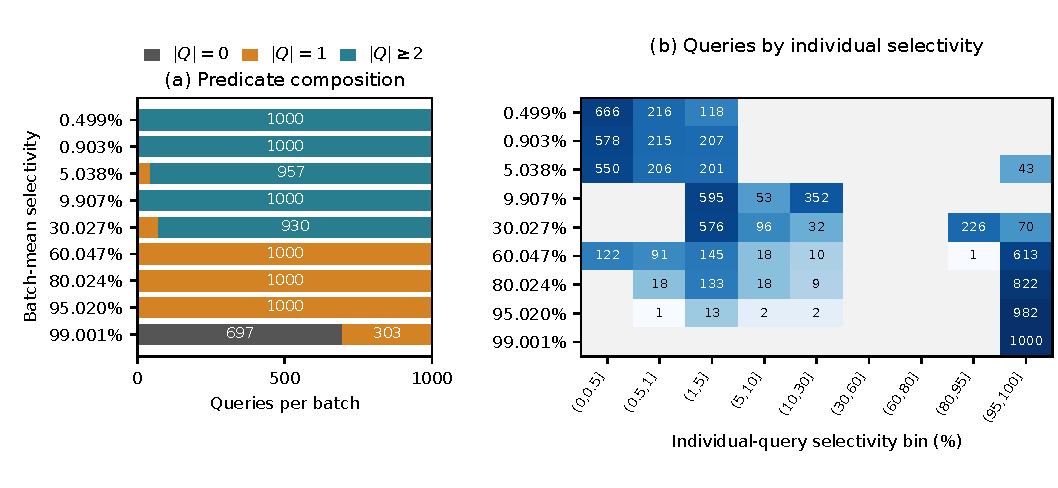
\includegraphics[width=\textwidth]{generated_figures/query_strata/query_composition.pdf}
\caption{Composition of the nine Amazon batches, each with 1,000 queries.
Left: number of predicate labels. Right: query counts by exact eligible-vector
fraction; bins are open on the left and closed on the right, and blank cells
contain no queries. Each row is labeled by its batch mean. A high mean can
coexist with many selective queries, and a singleton need not have high coverage.}
\label{fig:query-composition}
\end{figure*}

The five manual plans perturb the automatic two-overlay plan
$(t,16t)$: one LNG overlay at $t$; two LNG overlays at $(t,16t)$;
two Trie overlays at $(t,16t)$; and LNG/Trie overlays at
$(t/2,8t)$ or $(2t,32t)$. Here $t$ is 256 for Genome, 512 for
Reviews, and 1024 for VariousImg. All share the LNG base and the
presence gate used by DRH-v1; consequently the one-overlay alternative
always falls back to the base under this gate.

\subsection{Methods and Fairness}
The principal 0L comparison is LNG topology with optimized-LNG entry
discovery versus Trie topology with Trie entry discovery.  The topology
factorial fixes $T_1=1024$, $T_2=16384$, and ungated routing while enumerating
both base topologies and every LNG/Trie upper-layer assignment through 2L.
Within either base, replacing one upper letter is a controlled topology
comparison because its entry provider is unchanged.  Across bases we instead
report a matched-provider system comparison, not a pure edge-topology effect.
Routed controls are evaluated separately because routing changes the
executed search algorithm. For held-out automatic-policy evaluation, however,
the exact gate is fixed for DRH and every manual-alternative hierarchy; the
ungated DRH variant is reported separately.

We call the 0L LNG configuration \emph{Plain} or \emph{0L-LNG}.  It
preserves UNG's exact-label groups, LNG cover relation, and unified vector
graph, with our optimized, semantically equivalent minimal-superset
provider and the common refactored execution path.  Within a fixed LNG base and provider, this is the control for adding overlays.

Within each comparison, query methods use the same data, query vectors, labels, exact ground truth,
$K$, thread count, immutable search binary, graph backend, and Recall protocol.
Each case executes one cold and two warm repeats of the same frozen query
file in the same order. We discard the cold repeat and derive QPS from the
median warm batch time. The operating point is the smallest executed
$L_{search}$ for which both warm repeats reach batch-mean Recall@10 $\ge0.90$.
A separate instrumented pass collects stage times and work counters.
If a method has no screen crossing, its
crossing pass extends to the largest $L_{search}$ measured for any method on
that workload (or an explicitly declared common cap); only failure at that
shared budget is reported as no crossing.
The workload-specific search caps appear in Table~\ref{tab:budgets}.

\subsection{Metrics}
Table~\ref{tab:metric-definitions} in Appendix~\ref{sec:measurement-details}
defines all stage times and counters. Primary throughput is
$\mathrm{QPS}=1000B/\mathrm{batch\ latency\ (ms)}$.  Batch size $B$ is workload-specific: 1,000 on Amazon and
2,864 or 3,000 on the held-out workloads (Table~\ref{tab:heldout-datasets}).  Primary query metrics are
warm-median batch latency and QPS. With only two warm repeats, we report the observed throughputs
without query-performance confidence intervals.

Build timing uses process wall time through files on disk, followed by
structural acceptance checks; kernel time is never substituted for builder
wall time. The current construction evidence contains two measured repeats
per hierarchy backend, after a cold run, and a separate memory-resource pass.
The composed total adds independently measured base and sidecar stage medians.
We report observed dispersion across the two stage repeats.
GPU cases require three consecutive idle-device snapshots before timing. Backend counters and reload checks validate execution and structure.
These construction times compare the declared builders; query-quality
equivalence of their output graphs has not been measured.

The exact CPU/GPU routes are fixed before measurement; Appendix~\ref{sec:build-profiles}
lists the base and hierarchy profiles. They differ in local graph construction,
metadata preparation, and cross-edge generation, so their total-time ratios
measure complete builder profiles.

\section{Results}
The sweep compares selective-predicate batches and mixtures containing a
frequent singleton, using the batch-mean selectivity defined in Section~\ref{sec:methodology}.
\subsection{Matched Base and Overlay Choices}
\baseTopologyFixedConfigurations
Table~\ref{tab:fixed-topology-configurations} follows four unchanged
configurations through the nine Amazon batches. The fixed
\texttt{2L[T|LT]} improves on Plain in seven batches, while Plain leads
near 10\% and 30\%. It also permits a direct depth comparison against
\texttt{1L[T|L]}, without changing the base, provider, or first overlay.
These configurations are examined on the development dataset; the
held-out policy study below evaluates a different, fixed-LNG-base rule.
The complete grid and its per-workload winners appear in
Tables~\ref{tab:base-topology-winners}--\ref{tab:base-topology-factorial-b}.
\baseTopologyFactorialFindings

The original warm repeats also qualify the small depth differences.
For fixed \texttt{2L[T|LT]} versus \texttt{1L[T|L]}, the observed QPS ranges
overlap near 60\% and 80\%. Near 95\%, all four cross-repeat ratios lie
between 1.072 and 1.098. These describe the two recorded executions per
configuration; they are not confidence intervals. Table~\ref{tab:warm-repeat-ranges}
reports the ranges alongside exact selected capacities.

The selected search budget is part of the observed performance difference.
On the four batches near 60--99\%, Plain requires capacities of
260,000--400,000, whereas \texttt{2L[T|LT]} uses 1,000--5,000.
The array-queue term in Section~\ref{sec:query} makes those capacities
consequential for work as well as memory. The throughput ratios therefore
combine different navigation paths and the costs of their required search
budgets. Figure~\ref{fig:topology-grid} shows both quantities across the grid.

The LNG-minimal-entry overlays have no crossing on the five lower-mean
batches at these thresholds. Section~\ref{sec:retag-coverage} demonstrates
that their entry contract can lose coverage before any capacity limit is
applied. The recorded screen does not measure per-query exhaustive
reachability, so it cannot apportion these NCs between structural coverage
loss and finite-budget search.

\subsection{Recall Within the Batches}
Regrouping the original per-query records reconstructs all 190 warm batch
means and exposes variation hidden by the crossing criterion. In the
5.038\% batch, 43 queries share the singleton predicate $\{1\}$, which
admits 96.702\% of the database.
Their mean Recall is 28.84\% for Plain, 14.88\% for \texttt{0L[T]},
73.26\% for \texttt{1L[T|L]}, and 74.42\% for \texttt{2L[T|LT]} in both
warm executions. The fixed two-overlay configuration reaches 92.64\%
on the other 957, multilabel queries; four of its singleton queries have
zero Recall. Thus its batch crossing and throughput gain coexist with a
subgroup substantially below the target (Table~\ref{tab:query-size-recall}).

Predicate size alone does not identify the difficult subset. In the
30.027\% batch, \texttt{2L[T|LT]} reaches 94.57\% Recall on the 70
singletons, but only 66.81\% on the 226 multilabel queries whose individual
selectivity lies in $(80\%,95\%]$. All 226 share the predicate $\{1,2\}$,
which admits 91.055\% of the database. Plain reaches 71.64--74.29\% on that
latter subset (Table~\ref{tab:query-selectivity-recall}). Near 60\%, 80\%,
and 95\% batch-mean selectivity, the fixed two-overlay system has 31, 29,
and 33 zero-Recall queries per execution, versus 11--12, 12, and 14 for
Plain. These distributions retain each method's own batch-selected capacity;
they describe query-level quality at the reported throughput points, rather
than subgroup-matched Recall comparisons. The repeated predicates also
limit what these subsets establish about other predicates in the same bin.

\subsection{Where Discovery Savings Go}
\authoritativeAmazonSummary
The profiles expose the tradeoff behind the base comparison
(Figure~\ref{fig:motivation}). At 0.499\%, Trie reduces discovery from
20.352 to 0.645 ms/query, while seed setup rises from 0.195 to 1.769 ms.
Graph time also falls, from 2.076 to 0.868 ms. At 9.907\%, discovery still
falls, from 36.631 to 3.778 ms, but seed setup rises to 14.744 ms and graph
time increases from 98.747 to 323.081 ms. Cheaper entry discovery therefore
coincides with both a winning and a losing end-to-end configuration.
The changed frontier and topology shift work into different stages.

Blocks can recover throughput on batches with larger mean selectivity. Keeping the LNG base
and its optimized provider fixed, the ungated one-overlay system reaches
27.99$\times$ Plain and the two-overlay system reaches 27.57$\times$ on
the measured higher-mean-selectivity batches (Table~\ref{tab:amazon-depth}). Both fail
to cross at 30\% within the shared budget. In the full grid, the best
one-overlay system already leads at 60\% and 80\%; a second overlay is
useful at 95\%, where the best QPS rises from 520.35 to 564.63.
Thus additional scale can help, but the base, overlay topology, and seed
competition jointly determine its value.

\subsection{Automatic Policy Transfer}
\authoritativePolicyResults
DRH-v1 remains near Plain on Genome and Reviews (0.954--1.014$\times$),
but falls to 0.205$\times$ on VariousImg (Table~\ref{tab:heldout}). Its
ratios to the best of the five manual alternatives are 0.980--1.008 on
Genome/Reviews and 0.218 on VariousImg. A fixed structural plan therefore
transfers unevenly. The best manual candidate on VariousImg is the
one-overlay plan, whose presence gate executes base search; its advantage
there comes from rejecting the overlays.
The per-workload manual winner is selected in hindsight. Table~\ref{tab:heldout-global}
also compares one fixed plan per dataset, aggregated over its workloads.

The separate mass-gate experiment tests this failure mode. On VariousImg,
DRH-v2 raises QPS from 547.01 to 884.18, reaching 0.336$\times$ its
same-cohort Plain. On the 4.115\% Reviews workload it rejects a useful
overlay and falls to 0.972$\times$ Plain (Table~\ref{tab:drh-v2}).
Increasing the admission requirement reduces one regression but loses a
beneficial case.

The profiles show how routing changes work averaged over all queries
in each broader workload (Table~\ref{tab:profile}). On VariousImg, the multilayer backend is
active for 37.4\% of queries; mean scanned edges rise from 119,045.5 to
251,144.0 and graph time rises from 35.098 to 172.065 ms/query. On Reviews,
activation is 18.2\%, distances fall from 8,239.3 to 7,312.0, and graph time
changes from 6.756 to 6.504 ms/query. These contrasting outcomes motivate
an admission model that accounts for expected navigation work as well as
certifiable mass. All four datasets derive two overlays, so this experiment
examines scale and topology transfer at a fixed resulting depth.

\subsection{Construction Cost}
\authoritativeBuildResults
On Amazon, the fastest hybrid builder reduces hierarchy construction from
1000.64 to 90.49 seconds, an 11.06$\times$ ratio; the full-GPU route takes
105.90 seconds (Table~\ref{tab:hierarchy-build}). Adding GPU cross-edge
construction to the hybrid route increases time to 132.94 seconds, and the
TF32-WMMA route takes 1011.13 seconds. More GPU execution is therefore
not uniformly beneficial for these irregular tasks.

Including the separately measured accelerated base stage gives composed
times of 141.27 seconds for the fastest hybrid and 156.69 seconds for full
GPU, compared with 190.38 seconds for the original CPU base builder
(Table~\ref{tab:end-to-end-build}). The resulting ratios are 1.35$\times$
and 1.21$\times$. The hybrid resource pass records 4880.7 MiB peak host
RSS and 1598.0 MiB peak device allocation. Table~\ref{tab:sidecar-build}
reports the CPU sidecars used to enable the held-out query study.
